\documentclass[
]{thesis-ekf}
\usepackage[T1]{fontenc}
\PassOptionsToPackage{defaults=hu-min}{magyar.ldf}
\usepackage[magyar]{babel}
\usepackage{mathtools,amssymb,amsthm,pdfpages}
\usepackage{graphicx, url}
\usepackage{placeins}
\usepackage{float}
\usepackage{listings,xcolor,caption,upquote}
%\lstloadlanguages{JavaScript}
\footnotestyle{rule=fourth}

\newtheorem{tetel}{Tétel}[chapter]
\theoremstyle{definition}
\newtheorem{definicio}[tetel]{Definíció}
\theoremstyle{remark}
\newtheorem{megjegyzes}[tetel]{Megjegyzés}

\lstset{
	inputencoding=utf8/latin2,
	basicstyle=\footnotesize\ttfamily,
	columns=fullflexible,
	numbers=left,
	breaklines,
	postbreak=\hbox{$\mathcolor{red}{\hookrightarrow}$\ },
	xleftmargin=2cm,
	xrightmargin=2cm,
	frame=single,
	literate={ó}{\'{o}}1
	{á}{\'{a}}1
	{é}{\'{e}}1
	{í}{\'{i}}1,
}

\lstdefinestyle{myjavascript}{
	language=JavaScript,
	backgroundcolor=\color{cyan!10},
	keywordstyle=\color{blue},
	commentstyle=\itshape\color{teal},
	identifierstyle=\color{black},
	stringstyle=\color{red},
}

\lstdefinestyle{mypython}{
	language=Python,
	backgroundcolor=\color{cyan!10},
	keywordstyle=\color{blue},
	commentstyle=\itshape\color{teal},
	identifierstyle=\color{black}
}

\renewcommand{\lstlistingname}{kód}

\begin{document}
	
	\institute{Matematikai és Informatikai Intézet}
	\title{Személyi igazolványok digitális tárolása}
	\author{Kovács Gábor\\programtervező informatikus}
	\supervisor{Dr. Kovásznai Gergely\\Tanszékvezető, egyetemi docens}
	\city{Eger}
	\date{2025}
	\maketitle
	
	\tableofcontents
	
	\chapter*{Bevezetés}
	
	\chapter{Személyazonosítás fejlődése és digitalizációja}
	
	\section{A személyi igazolványok története}
	
	Ebben a fejezetben röviden végigmegyünk a személyazonosító igazolványok történetén. A személyazonosítás igénye évezredekre nyúlik vissza, hiszen a társadalmak mindig is szerették volna hiteles módon azonosítani tagjaikat. Az ókori birodalmakban pecsétes levelek, ujjlenyomatos agyagpecsétek és különböző azonosító jegyek szolgáltak erre a célra.  A középkorban a nemesi kiváltságokat vagy állampolgárságot igazoló dokumentumokat használtak, például a pápai bullákat vagy a királyi rendeleteket. \cite{okoriAzonositas, kozepkorAzonositas}
	
	A modern értelemben vett személyi igazolványok a 19. és 20. században terjedtek el, amikor az államok egyre inkább szükségét érezték annak, hogy állampolgáraikat hivatalos dokumentumokkal azonosítsák. Magyarországon az első személyi igazolványokat a második világháború után vezették be, és azóta számos változáson mentek keresztül, mind biztonsági, mind technológiai szempontból. \cite{magyarAzonositas}
	
	\section{A digitális azonosítás megjelenése}
	A 21. században a digitális technológia fejlődésével a személyazonosítás egyre inkább az elektronikus rendszerekre helyeződött át. Az internet elterjedésével növekedett az igény a biztonságos online azonosításra, amely a hagyományos személyi igazolványok digitális megfelelőit hívta életre.
	
	Számos országban, mint például Észtországban bevezették az elektronikus személyi igazolványokat (eID), amelyek beépített chippel rendelkeznek, és különböző biometrikus adatokat is tárolhatnak, mint ujjlenyomat vagy arcfelismerési információ. Ezek az azonosítási módszerek jelentősen javítják a biztonságot és megkönnyítik az online szolgáltatásokhoz való hozzáférést. \cite{magyarAzonositas}
	
	\section{A mobiltechnológia és az azonosítás}
	Az okostelefonok és a mobilalkalmazások terjedésével az azonosítás folyamata tovább egyszerűsödött. A felhasználók ma már egyetlen kattintással vagy biometrikus azonosítással (pl. Face ID, ujjlenyomat-olvasó) hitelesíthetik magukat különböző szolgáltatásokhoz.
	
	A mobiltechnológia lehetővé tette a digitális személyazonosítás gyorsabb, kényelmesebb és biztonságosabb formáit. A blockchain\footnote{Az adatok ,,blokkokba'' vannak tárolva, amelyek egymáshoz vannak láncolva, így egy folyamatos, biztonságos láncot alkotnak.} alapú azonosítási rendszerek pedig tovább fokozzák az adatok védelmét, lehetőséget adva a felhasználóknak, hogy nagyobb kontrollt gyakoroljanak személyes adataik felett.
	
	\section{A digitalizáció jövője a személyazonosításban}
	A jövőben a személyazonosítás módszerei tovább fejlődnek, egyre inkább az automatizált és AI-alapú rendszerek irányába. Az arcfelismerés, a hangalapú azonosítás egyre népszerűbbé válik.
	
	A digitális személyazonosítás előnye, hogy gyorsabb és hatékonyabb az offline módszereknél, ugyanakkor komoly adatbiztonsági kihívásokat is felvet. A jövő fejlesztései során kulcsfontosságú lesz a magánszféra védelme és az etikus adatkezelés biztosítása.
	
	A digitális személyi igazolványok az állampolgárok azonosításának egyre népszerűbb eszközei világszerte. Ezek az okmányok nemcsak a hagyományos, fizikai igazolványok elektronikus megfelelői, hanem további funkciókkal is rendelkezhetnek, például online hitelesítésre, elektronikus aláírásra vagy egyes állami és magánszolgáltatások elérésére.
	
	Bár a digitális személyazonosítás rengeteg előnyt kínál, számos kihívás is társul hozzá, amelyek megoldása kulcsfontosságú a széleskörű elterjedéshez.
	\section{Előnyök}
	
	A digitális személyi igazolványok lehetővé teszik az azonosítás és hitelesítés gyors és kényelmes módját. Az állampolgárok anélkül igazolhatják magukat, hogy fizikai okmányt kellene magukkal hordaniuk, hiszen az azonosító adatok tárolhatók egy mobiltelefonon vagy egy biztonságos szerveren. Magyarországon a DÁP\footnote{Digitális Állampolgárság Program} valósítja ezt meg.
	
	Például egy e-személyi igazolvány segítségével egy banki ügyintézés vagy egy online regisztráció néhány kattintással elvégezhető, míg a hagyományos személyazonosítás esetében papírokat kell kitölteni, aláírni és személyesen bemutatni.

	A digitális személyazonosító igazolványok a legmodernebb titkosítási technológiákat alkalmazzák, így nehezebben hamisíthatók, mint a hagyományos plasztikkártyák. Egy jól megtervezett digitális rendszerben az adatok ellenőrzése és tárolása szigorú biztonsági szabványok szerint történik, csökkentve az illetéktelen hozzáférés vagy visszaélés esélyét. Az Európai Unióban az Európai Bizottság felelős a digitális személyazonosításra vonatkozó szabályozásért, melynek keretében az eIDAS és az EUDI rendeletek meghatározó szerepet töltenek be a biztonságos digitális azonosítási keretrendszer kialakításában. \cite{eIDAS, EUDI}
	
	Biometrikus azonosítókkal (például arcfelismerés vagy ujjlenyomat) kombinálva az e-személyik még biztonságosabbá válhatnak, hiszen a felhasználó azonosítása egyértelmű és nehezen másolható.

	A digitális személyi igazolványok hozzájárulhatnak a papíralapú ügyintézés csökkentéséhez, ami nemcsak a környezetvédelmet szolgálja, hanem a közigazgatási rendszerek hatékonyságát is növeli. A kevesebb nyomtatás, postázás és manuális adatfeldolgozás hosszú távon jelentős költségmegtakarítást eredményezhet az állam és a vállalatok számára is.
	\section{Kihívások}

	A digitális személyazonosító rendszerek egyik legnagyobb kihívása az adatbiztonság. Mivel ezek az igazolványok személyes adatokat tartalmaznak, kiemelt célpontjai lehetnek kibertámadásoknak és adatlopásoknak. Egy esetleges rendszerfeltörés vagy adatvédelmi incidens súlyos következményekkel járhat az érintettek számára.
	
	Ennek elkerülése érdekében olyan technológiákat kell alkalmazni, mint a többfaktoros hitelesítés, az adatok titkosítása és a decentralizált adattárolás. Az adatvédelmi jogszabályok is szigorúan szabályozzák, hogy a digitális személyi igazolványokhoz kapcsolódó információkat hogyan lehet kezelni és tárolni.

	Bár a digitális személyi igazolványok kényelmesek lehetnek a technológiailag fejlett országokban, nem mindenki fér hozzá megfelelő eszközökhöz vagy internetkapcsolathoz. Az idősebb generációk, a technológiai ismeretekkel kevésbé rendelkezők vagy a hátrányos helyzetű régiókban élők számára nehézséget jelenthet az új rendszer használata.
	
	Emellett az infrastruktúrának is fel kell készülnie a digitális személyazonosítás kezelésére. Például egy digitális személyi igazolvány csak akkor használható széles körben, ha az intézmények és vállalkozások rendszerei kompatibilisek vele.

	A digitális azonosítás jogi szabályozása még sok helyen gyerekcipőben jár. Az eltérő nemzeti szabályozások és az adatvédelmi törvények miatt nehéz olyan univerzális rendszert kialakítani, amely minden országban elfogadott és kompatibilis lenne a helyi előírásokkal.
	
	Például egy olyan digitális személyi igazolvány, amely egy adott országban teljes körű hitelesítésre képes, nem biztos, hogy egy másik országban is elfogadott. A nemzetközi standardok és együttműködések kialakítása kulcsfontosságú lehet a rendszer globális elterjedése szempontjából.
	
	\chapter{A mesterséges intelligencia szerepe az adatfeldolgozásban}
	A mesterséges intelligencia (MI) forradalmasította az adatfeldolgozást és az automatizált döntéshozatalt. A hagyományos, manuális adatrögzítési módszerekkel szemben az MI-alapú rendszerek képesek nagy mennyiségű információ gyors és pontos feldolgozására, ami különösen hasznos a dokumentumok digitalizálása és azonosítási rendszerek fejlesztése terén.
	
	\section{Mi az az OCR (Optikai karakterfelismerés)?}
	Az Optical Character Recognition (OCR) egy olyan technológia, amely képes nyomtatott vagy kézírásos szövegeket digitális formátumba alakítani. Az OCR segítségével az igazolványokról készült fényképeken található szöveg gépileg olvasható formátummá konvertálható, így az adatok feldolgozása és tárolása automatizálható.
	
	Az OCR működésének lépései:
	\begin{enumerate}
		\item \textbf{Kép előfeldolgozása} -- A képből eltávolítják a zajokat (például árnyékokat vagy torzításokat), hogy a karakterek élesebben felismerhetők legyenek.
		\item \textbf{Karakterek felismerése} -- Az MI-alapú OCR rendszerek neurális hálók segítségével azonosítják az egyes betűket és számokat.
		\item \textbf{Szöveg átalakítása és értelmezése} -- A felismerés után a szöveget szerkezetileg elemzik, hogy a megfelelő adatokat lehessen kinyerni belőle (például név, születési dátum, igazolványszám).
	\end{enumerate}
	
	Az ilyen rendszerek \textbf{gépi tanulással} folyamatosan fejleszthetők: minél több igazolványt dolgoznak fel, annál pontosabb lesz a felismerés és az adatkivonás.
	
	\section{Hogyan segíthet az MI a dokumentumok feldolgozásában?}
	A mesterséges intelligencia a dokumentumfeldolgozás több aspektusában is jelentős segítséget nyújt:
	\begin{itemize}
		\item \textbf{Automatizált adatkinyerés} -- Az MI-alapú rendszerek az igazolványokról gyorsan és pontosan kivonják az adatokat, csökkentve a manuális bevitel szükségességét.
		\item \textbf{Hibajavítás és adatellenőrzés} -- Az MI képes felismerni és javítani a karakterfelismerési hibákat, valamint ellenőrizni az adatok érvényességét (pl. egy születési dátum valós lehet-e).
		\item \textbf{Biztonsági ellenőrzések} -- Az MI algoritmusok kiszűrhetik a hamis vagy manipulált igazolványokat azáltal, hogy összehasonlítják azokat ismert mintákkal és adatbázisokkal.
		\item \textbf{Adatvédelmi és titkosítási megoldások} -- Az MI segítségével érzékeny személyes adatok anonim módon tárolhatók és dolgozhatók fel, csökkentve az adatlopás kockázatát.
	\end{itemize}
	\section{A mesterséges intelligencia jövője az adatfeldolgozásban}
	Ahogy az MI-technológiák egyre fejlettebbé válnak, az adatfeldolgozás pontossága és hatékonysága tovább javulhat. A jövőben várható fejlesztések közé tartozik:
	\begin{itemize}
		\item \textbf{Még pontosabb OCR és természetes nyelvfeldolgozás (NLP)} -- Az MI képes lesz még bonyolultabb dokumentumokat is pontosan értelmezni.
		\item \textbf{Valós idejű adatfeldolgozás} -- Az azonosítási folyamatok azonnali ellenőrzése és feldolgozása még gyorsabbá válhat.
		\item \textbf{Blokklánc és decentralizált identitáskezelés} -- Az MI és a blokklánc kombinálásával a személyazonosító adatok még biztonságosabbá tehetők.
	\end{itemize}
	Összességében a mesterséges intelligencia egyre fontosabb szerepet tölt be a személyazonosító dokumentumok digitális feldolgozásában. Az automatizálás, a pontosság és a biztonság növelésével hozzájárul ahhoz, hogy a felhasználók kényelmesebben és gyorsabban intézhessék ügyeiket a digitális világban.
	
	\chapter{Neurális hálók}
	
	A mély neurális hálózatok több egymásra épülő rétegből állnak, amelyek mesterséges neuronokat vagy csomópontokat tartalmaznak. \Aref{fig-neural} ábrán szemléltetett módon ezek a csomópontok különböző matematikai műveleteket végeznek el, jellemzően lineáris transzformációkat, amelyek révén az információ feldolgozása és továbbítása történik.
	
	\begin{figure}
		\centering
		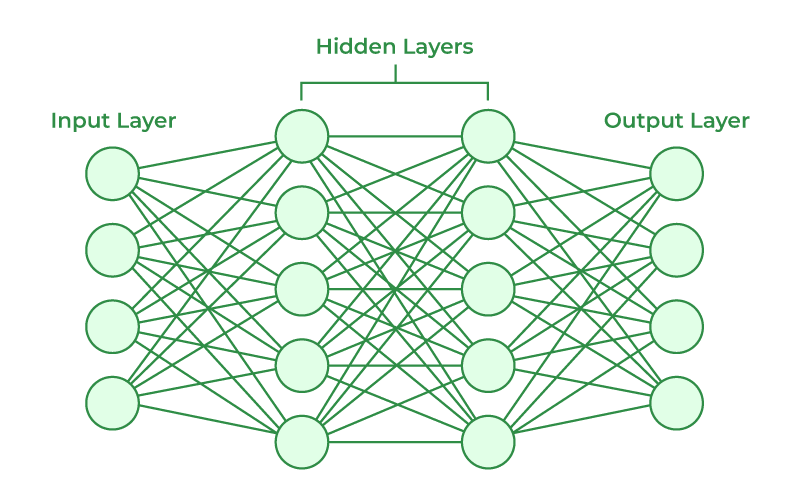
\includegraphics[width=10cm]{Neural-Networks-Architecture}
		\caption{Neurális háló, forrás: \cite{neuralNetworkImage}}
		\label{fig-neural}
	\end{figure}
	
	Ezek a hálózatok három fő rétegből épülnek fel: a bemeneti rétegből, a rejtett rétegekből és a kimeneti rétegből. Az első réteg, a bemeneti réteg, fogadja és előkészíti az adatokat, amelyeket aztán a rendszer a következő szintek felé továbbít. A köztes rétegek, az úgynevezett rejtett rétegek, az adatok feldolgozását végzik. Ezek a rétegek az információkat nemlineáris aktivációs függvények segítségével alakítják át, és fokozatosan kinyerik a releváns jellemzőket a bemenetekből. \cite{neuralNetwork}
	
	A rejtett rétegek működése közvetlenül nem megfigyelhető, mivel a bennük található paraméterek – azaz a súlyok és eltolások – a tanulási folyamat során finomhangolódnak. Ezek a paraméterek lehetnek kezdetben véletlenszerűek, de előfordulhat, hogy előre meghatározott értékekkel indulnak, amelyeket korábbi tanulási tapasztalatok alapján állítottak be. A rejtett rétegek célja, hogy az adatok összetett mintázatait felismerjék és olyan jellemvonásokat azonosítsanak, amelyek hozzájárulnak a végső döntések meghozatalához, például egy predikció vagy osztályozás formájában. \cite{neuralNetwork}
	
	A rejtett rétegek által előállított információ végül eljut a kimeneti réteghez, amely a hálózat végső eredményeit biztosítja. Az adott feladattól függően ez a réteg lehetővé teszi az osztályozást, előrejelzést vagy akár új minták generálását. Az adatok ilyen módon történő feldolgozását és továbbítását előreterjesztésnek nevezzük, amely \aref{fig-neural}. ábrán is szemléltetett módon zajlik. \cite{neuralNetwork}
	
	\section{TensorFlow – A Mélytanulási Keretrendszer}
	
	A TensorFlow egy nyílt forráskódú, fejlett gépi tanulási és mesterséges intelligencia (AI) keretrendszer, amelyet a Google fejlesztett ki és tett elérhetővé 2015-ben. Az egyik legnépszerűbb eszközként szolgál a mesterséges intelligencia alkalmazások fejlesztésében, különösen a mélytanulási modellek létrehozásában. A TensorFlow egy olyan rugalmas és hatékony platform, amely lehetővé teszi a kutatók és fejlesztők számára, hogy széleskörű gépi tanulási modelleket és alkalmazásokat hozzanak létre és futtassanak különböző környezetekben, beleértve a felhőt, a mobil eszközöket és a beágyazott rendszereket.
	
	A TensorFlow kifejlesztésének fő célja, hogy megkönnyítse a gépi tanulás modellek létrehozását és implementálását, ugyanakkor a számítási feladatokat egy skálázható, párhuzamosítható grafikus számítási modellben kezelje. Az eszközt eredetileg a Google Brain csapata készítette, hogy támogassa a Google-hoz tartozó projektek, például a keresőoptimalizálás, képfeldolgozás, gépi fordítás, és más mesterséges intelligencia alkalmazások fejlesztését.
	
	A TensorFlow támogatja a különböző gépi tanulási algoritmusokat, mint például a felügyelt és felügyelet nélküli tanulás, valamint a mélytanulás különböző típusait, mint a neurális hálózatok, konvolúciós neurális hálózatok (CNN) és rekurzív neurális hálózatok (RNN). A TensorFlow képes hatékonyan futtatni modelleket CPU-n, GPU-n és más dedikált hardvereken, mint például a Tensor Processing Unit (TPU), amely a Google által kifejlesztett egyedi hardver az AI számítási feladatok gyorsítására.
	
	A TensorFlow egyik legnagyobb előnye az, hogy skálázható, tehát képes kis mértékű alkalmazásoktól kezdve, a világ legnagyobb felhőalapú rendszereit is kiszolgálni. Emellett a TensorFlow lehetővé teszi a modellek mobil eszközökön való futtatását, így a fejlesztők egyszerűen vihetik a mélytanulási megoldásaikat a mobil alkalmazások világába is.
	
	
\chapter{Backend-en használt technológiák}

\section{Node.js}	
A backend fejlesztés kulcsszerepet játszik a modern web- és mobilalkalmazások működésében, hiszen ezen a rétegen történik az adatok kezelése, tárolása és kiszolgálása. A szerveroldali technológiák közül a Node.js az egyik legnépszerűbb választás, amely lehetőséget biztosít arra, hogy az alkalmazás teljes fejlesztése JavaScript nyelven történjen. A Node.js egy gyors és hatékony futtatókörnyezet, amely eseményvezérelt és nem blokkoló működésének köszönhetően különösen alkalmas nagy teljesítményt igénylő alkalmazások készítésére.

\subsection{A Node.js alapjai és működési modellje}

A Node.js a Google V8 JavaScript motorjára épül, amely lehetővé teszi a JavaScript kód gyors végrehajtását szerveroldalon. Az egyik legfontosabb sajátossága az aszinkron és eseményvezérelt működés, amely lehetővé teszi, hogy a szerver egyszerre több kérést is kezeljen anélkül, hogy az egyes műveletek blokkolnák egymást. Mivel a Node.js nem használ többszálú feldolgozást, hanem egyetlen szálon fut, a skálázhatóságot egy úgynevezett eseményhurok biztosítja, amely a beérkező kéréseket folyamatosan fogadja és kezeli.

Az aszinkron működés egyik alapvető eszköze a visszahívási függvények (callback), amelyeket később az ígéretek (Promises) és az async/await konstrukciók egészítettek ki. Az alábbi példa bemutatja, hogyan lehet egy fájl beolvasását aszinkron módon végrehajtani a fs modul segítségével:

%\lstinputlisting[style=myjavascript,caption=Egy Node.js kód,label=kod-nodejs1]{nodejs_1.js}

Ebben a kódrészletben a fájl beolvasása nem blokkolja a többi művelet végrehajtását, mivel az eredmény egy visszahívási függvényben kerül feldolgozásra. Ennek köszönhetően a szerver továbbra is képes új kérések kiszolgálására, miközben a fájl beolvasása háttérben történik.

\subsection{A Node.js előnyei és kihívásai}
A Node.js egyik legnagyobb előnye a teljesítménye és skálázhatósága. Az eseményvezérelt architektúra miatt a szerver könnyedén kezelhet nagy számú egyidejű kapcsolatot anélkül, hogy túlterhelődne. Ez különösen előnyös olyan alkalmazások esetében, amelyek valós idejű interakciót igényelnek, például csevegőalkalmazások vagy élő adatstreaming megoldások.

Egy másik fontos előny a JavaScript használata mind a frontend, mind a backend fejlesztés során. Ez lehetővé teszi, hogy a fejlesztőcsapatok egységes technológiai környezetben dolgozzanak, ami jelentősen csökkenti a fejlesztési időt és egyszerűsíti a kód karbantarthatóságát.

A Node.js azonban nem minden esetben ideális választás. A CPU-intenzív műveletek, például nagy mennyiségű számítási feladatokat végző algoritmusok vagy mesterséges intelligencia modellek futtatása esetén a Node.js teljesítménye korlátozott lehet. Mivel egyszálú környezetben működik, a nagy számítási igényű feladatok blokkolhatják az egész szerver működését. Ilyen esetekben érdemes külső szolgáltatásokat vagy külön szálakon futó háttérfolyamatokat használni a terhelés elosztására.

\subsection{Backend fejlesztés Express.js segítségével}

A Node.js önmagában is alkalmas szerverek létrehozására, de a fejlesztést jelentősen megkönnyíti az Express.js, amely egy minimalista és rugalmas webkeretrendszer. Az Express lehetőséget biztosít API végpontok kialakítására, HTTP kérések kezelésére és middleware-ek használatára.

Az alábbi példában egy egyszerű szerver hozható létre Express segítségével, amely egy alapvető GET végpontot biztosít:

%\lstinputlisting[style=myjavascript,caption=Egy Node.js kód,label=kod-nodejs2]{nodejs_2.js}

Ez a kód mindössze néhány sorban egy működőképes HTTP szervert hoz létre, amely egy egyszerű üzenetet küld vissza a kliensek számára. Az Express egyik nagy előnye, hogy lehetővé teszi az útvonalak és middleware-ek könnyű kezelését, amelyek segítségével az alkalmazás bővíthető és testreszabható.

\subsection{Adatbázis-kezelés Node.js-ben}

A backend fejlesztés egyik alapvető feladata az adatkezelés, amelyhez különböző adatbázisokat lehet használni. A Node.js kompatibilis mind a relációs (SQL), mind a NoSQL adatbázisokkal. A relációs adatbázisok, például a MySQL vagy a PostgreSQL strukturált adatkezelést biztosítanak, míg a NoSQL megoldások, mint a MongoDB, rugalmasabb adatmodellezést tesznek lehetővé.

Egy MongoDB alapú adatbázis kapcsolat létrehozására a Mongoose csomag használható, amely egy objektumorientált adatmodellezést biztosító eszköz. Az alábbi példa egy egyszerű kapcsolat létrehozását és egy új adatrekord mentését mutatja be:

%\lstinputlisting[style=myjavascript,caption=Egy Node.js kód,label=kod-nodejs3]{nodejs_3.js}

A Mongoose használata lehetővé teszi az adatbázis-interakciók egyszerű kezelését, miközben biztosítja az adatok validálását és strukturálását. Az objektumorientált modellnek köszönhetően a JavaScript objektumok könnyedén átalakíthatók adatbázis-bejegyzésekké.

\section{MongoDB}

A MongoDB egy nyílt forráskódú, dokumentum-orientált adatbázis-kezelő rendszer (DBMS), amelyet a MongoDB, Inc. fejlesztett. Az adatokat dokumentumok formájában tárolja, amelyek általában JSON-szerű BSON formátumban (Binary JSON) kerülnek mentésre. Ez lehetővé teszi, hogy az adatokat rugalmasan, skálázható módon tároljuk, így ideális választás nagy mennyiségű, változó szerkezetű adat kezelésére.

A MongoDB-t 2007-ben alapították, és gyorsan elnyerte a fejlesztők és cégek körében a népszerűséget a hagyományos relációs adatbázisokkal szembeni előnyei miatt. Mivel a MongoDB nem követeli meg a szigorú séma használatát, az adatokat szabadon, dinamikusan tárolhatjuk, amely különösen hasznos a gyorsan változó vagy nem strukturált adatokkal dolgozó alkalmazások számára.

A MongoDB-t széles körben használják különböző típusú alkalmazásokban, beleértve a webalkalmazásokat, analitikai platformokat, valamint a Big Data és a gépi tanulási megoldásokat is. Különösen alkalmas a NoSQL adatbázisok közé tartozik, amelyek az újabb alkalmazásfejlesztési igényeknek megfelelően nem használják a relációs adatmodellek korlátait, például az előre meghatározott táblákat és a szigorú séma-rendszert.

\subsection{A MongoDB működési elve}
A MongoDB működésének alapja a dokumentum-orientált adattárolás. A dokumentumok egyszerű kulcs-érték párokat tartalmaznak, de sokkal összetettebb adatstruktúrákat is képesek tárolni, például tömböket, beágyazott dokumentumokat és más összetett típusokat. Az adatok nem táblákban és sorokban, hanem dokumentumokban vannak tárolva, amelyek egy-egy adatbázison belül kollekciókban helyezkednek el.

A MongoDB által használt adatmodell lehetővé teszi az adatbázisok szabad struktúráját, amely rugalmasságot biztosít a fejlesztők számára, hiszen nem szükséges előre definiálni az adatbázis séma szerkezetét. Ez különösen hasznos akkor, amikor az adatok változnak, fejlődnek vagy különböző forrásokból származnak.

Mivel a MongoDB adatokat dokumentumokban tárolja, amelyek JSON-szerű formátumban vannak, az adatok hierarchikus struktúrában szervezhetők. Az adatmodell nemcsak a gyors fejlesztést és a rugalmas adattárolást teszi lehetővé, hanem a különböző adatfeldolgozási műveletek (például lekérdezések, frissítések, törlés) egyszerűsítését is.

\subsection{A MongoDB Különleges Jellemzői}
A MongoDB kiemelkedő jellemzője a skálázhatóság, amely lehetővé teszi a rendszer számára, hogy adatokat nagy mennyiségben kezeljen anélkül, hogy teljesítménybeli problémák merülnének fel. A MongoDB többféle skálázási lehetőséget kínál, mint például a sharding, amely az adatokat több szerverre osztja el, és a replikáció, amely biztosítja az adatok biztonságos és megbízható tárolását.

A sharding azt jelenti, hogy a MongoDB képes az adatokat különböző szerverek között megosztani (például egy szétosztott rendszerben), így képes nagyobb adatbázisokat kezelni. Mindez a rendszer teljesítményét nem befolyásolja, mivel minden egyes szerver csak egy részét tárolja az adatoknak. A replikáció segítségével a MongoDB biztosítja az adatok elérhetőségét, mivel az adatok több példányban vannak tárolva, és ezek automatikusan szinkronizálódnak a szerverek között. Ez a mechanizmus biztosítja az adatbázisok megbízhatóságát és rendelkezésre állását.

A másodlagos indexek és a full-text keresés lehetővé teszik a MongoDB számára, hogy gyorsan és hatékonyan végezzen kereséseket az adatok között, így megfelelő választ adva a komplex lekérdezési igényekre is. Az indexek a lekérdezések sebességét növelik, míg a full-text keresés lehetővé teszi a szöveges adatok gyors feldolgozását.

\subsection{A MongoDB Előnyei és Hátrányai}

Mivel a MongoDB nem követeli meg a szigorú séma alkalmazását, lehetőséget biztosít a változó adatstruktúrák kezelésére. Az adatbázis szerkezete bármikor változtatható, új mezők és adatpontok hozzáadása nem igényel az egész adatbázis átdolgozását.

A MongoDB képes hatékonyan kezelni nagy mennyiségű adatot, akár több szerverre is szétosztva a sharding mechanizmus segítségével, így biztosítva a magas rendelkezésre állást és megbízhatóságot.

A MongoDB gyors adatolvasást és -írást biztosít, különösen a nagy mennyiségű, változatos adatokat kezelő alkalmazások esetében.

A MongoDB rugalmas adatmodellt kínál, amely lehetővé teszi a gyors iterációt és az alkalmazások gyors fejlesztését. A séma nélküli adatbázisok különösen hasznosak olyan dinamikus alkalmazások esetén, ahol az adatok gyorsan változnak.

Bár a MongoDB folyamatosan fejlődik ezen a téren, a relációs adatbázisokhoz képest még mindig gyengébb a tranzakciókezelés, különösen komplex, több lépéses tranzakciók esetén.

Mivel a MongoDB nem használja a hagyományos relációs adatbázisokat, a fejlesztőknek nem minden esetben van elegendő tapasztalatuk ezzel a technológiával, és bár a közösség növekszik, még mindig kisebb, mint a hagyományos adatbázisoké.

Mivel a MongoDB nem használ előre meghatározott sémát, az adatok szerkezete nem mindig van megfelelően standardizálva, ami problémákat okozhat a nagy rendszerek integrálásakor.

\subsection{A MongoDB Alkalmazásai}
A MongoDB különösen akkor válik hasznossá, amikor az alkalmazás olyan Big Data vagy valós idejű adatfeldolgozási igényekkel rendelkezik, amelyek nagy volumenű és folyamatosan változó adatokat igényelnek. Ilyen típusú alkalmazások közé tartoznak például a webalkalmazások, mobilalkalmazások, e-kereskedelmi rendszerek, big data elemzések, valamint az IoT rendszerek. A MongoDB nagy sebességű, dinamikus adatfeldolgozási képessége miatt ideális választás olyan modern alkalmazásokhoz, amelyek gyorsan reagálnak az adatváltozásokra, és nem igényelnek szigorú adatmodell-szerkezetet.

\chapter{Frontend-en használt technológiák}
\section{React Native}

A React Native egy nyílt forráskódú keretrendszer, amelyet a Facebook fejlesztett ki, és amely lehetővé teszi natív mobilalkalmazások fejlesztését JavaScript és React használatával. A React Native célja, hogy egyszerűsítse a mobilalkalmazások fejlesztését, miközben a natív alkalmazások teljesítményét és élményét biztosítja. A keretrendszer alapja a React, amely egy JavaScript könyvtár a felhasználói felületek (UI) építésére, de a React Native lehetővé teszi, hogy ugyanazt a kódot használjuk mind az Android, mind pedig az iOS platformokon. Ez különösen vonzó azoknak a fejlesztőknek, akik keresnek egy költséghatékony és időtakarékos megoldást a mobilalkalmazások fejlesztésére.

\subsection{A React Native Működési Elve}

A React Native működésének alapja a natív komponensek és JavaScript köteg kombinációja. Amíg a React webalkalmazásoknál HTML és CSS használatával építi fel a felhasználói felületet, addig a React Native natív iOS- és Android-komponenseket használ. Ez azt jelenti, hogy bár a fejlesztő JavaScript-ben írja meg a kódot, a végén az alkalmazás natív komponensekben jelenik meg a mobil eszközökön, így biztosítva a natív alkalmazásokhoz hasonló teljesítményt és élményt.

A React Native alkalmazások a következőképpen működnek:
\begin{itemize}
	\item JavaScript szál: Az alkalmazás logikáját és az állapotkezelést JavaScript kódban valósítják meg, amely a React-tel működik. Ez a kód kezelni fogja az eseményeket, az adatokat, és irányítja a felhasználói felületet.
	\item Natív szál: A React Native alkalmazások natív szálat használnak az Android és iOS platformok natív komponenseihez való hozzáféréshez. Az alkalmazás natív elemei, mint például a gombok, szövegdobozok, listák és más UI komponensek, teljes mértékben az adott platform natív funkcióit használják.
\end{itemize}

Ez a megoldás lehetővé teszi, hogy a fejlesztők a natív alkalmazások sebességét és reakcióképességét érjék el, miközben csak egy kódot kell írniuk mindkét platformra.

\subsection{A React Native Jellemzői}

A React Native több fontos jellemzőt kínál, amelyek a modern mobilalkalmazások fejlesztésének alapvető szükségleteit szolgálják ki. Ezek közé tartozik a gyors fejlesztés, a natív élmény, az eszközökhöz való közvetlen hozzáférés és a közösségi támogatás.

A keretrendszer egyik legnagyobb előnye, hogy ugyanazt a JavaScript kódot használhatjuk az Android és iOS alkalmazásokhoz is. Ez jelentős időt és erőforrást takarít meg, mivel nem szükséges különböző nyelveken és fejlesztési környezetekben dolgozni a két platform számára. Az alkalmazás üzleti logikáját és felhasználói felületét ugyanazon a kódalapú megoldáson fejleszthetjük, így a fejlesztési ciklusok gyorsabbak és hatékonyabbak lesznek.

Bár a React Native egy JavaScript alapú keretrendszer, a natív komponensek használatának köszönhetően az alkalmazások teljesítménye közel áll a natív alkalmazásokéhoz. A keretrendszer lehetőséget ad arra, hogy közvetlenül hozzáférjünk az eszköz hardveréhez és szoftveréhez, mint például a kamera, a GPS, az érintőképernyő és más natív API-k. Ezen kívül lehetőség van natív modulok létrehozására, amelyek még jobb teljesítményt biztosítanak a kritikus alkalmazás részek számára.

A React Native mögött hatalmas fejlesztői közösség áll, amely folyamatosan bővíti és fejleszti a keretrendszert. Ennek eredményeként számos könyvtár és eszköz érhető el, amelyek segíthetnek a gyakori feladatok, mint például az adatkezelés, a navigáció vagy az animációk kezelésében. A közösség által nyújtott támogatás rendkívül hasznos a fejlesztők számára, mivel gyorsan válaszokat és megoldásokat találhatnak a problémákra.

\chapter{A projekt}

A projekt célja egy olyan mobilalkalmazás fejlesztése volt, amely lehetőséget biztosít a felhasználók számára személyazonosságuk igazolására. A rendszer működése során a felhasználó először regisztrál az alkalmazásban, majd ezt követően a személyazonosító okmányáról egy fényképet készít. Az így kapott kép feldolgozása egy neurális hálózat segítségével történik, amely azonosítja és kinyeri a releváns adatokat az okmányról. Az így kinyert információkat az alkalmazás egy biztonságos adatbázisban tárolja, biztosítva ezzel a felhasználó azonosításának megbízhatóságát és hatékonyságát.

\section{Adathalmaz generáló program}

A neurális háló hatékony betanításához megfelelő mennyiségű és változatosságú adathalmazra (dataset) volt szükség. Mivel nem létezett olyan nyilvánosan elérhető adatforrás, amely magyar személyazonosító igazolványok képeit tartalmazta volna, ezért a szükséges adatkészletet saját magamnak kellett előállítanom. Az adathalmaz generálása során az alábbi lépéseket követtem.

Az első lépés egy megfelelő alapként szolgáló személyazonosító igazolvány képének beszerzése volt. Az interneten keresve találtam egy olyan példányt, amely megfelelő referenciát biztosított a további példányok előállításához. Az így kiválasztott minta \aref{fig-eszemelyi} ábrán látható:

\FloatBarrier
\begin{figure}[H]
	\centering
	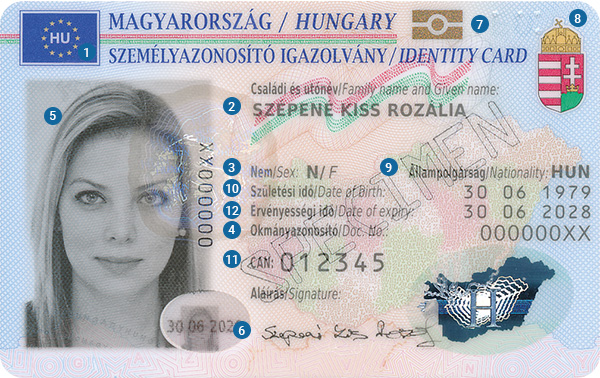
\includegraphics[width=8cm]{eszemelyi-front}
	\caption{Minta személyazonosító igazolvány, forrás: \cite{eszemelyiImage} }
	\label{fig-eszemelyi}
\end{figure}

Mivel az eredeti képen valós személyes adatok szerepeltek, ezért azokat el kellett távolítanom. Ehhez az Adobe Photoshop szoftvert használtam, amellyel kitöröltem az összes szöveget és egyéb személyes információt, így egy üres, adatmentes igazolványt kaptam. A megtisztított igazolvány \aref{fig-eszemelyi-photoshopped} ábrán tekinthető meg:

\FloatBarrier
\begin{figure}[H]
	\centering
	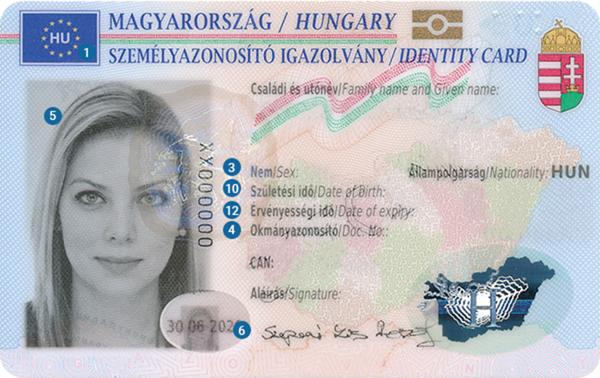
\includegraphics[width=8cm]{eszemelyi-front_photoshopped}
	\caption{Minta személyazonosító igazolvány retusálva, forrás: saját kép }
	\label{fig-eszemelyi-photoshopped}
\end{figure}

\begin{lstlisting}[style=mypython,caption=Augmentáció és fájlmentés, label=kod-python1]
	def generate_random_date(start_date, end_date):
	random_days = random.randint(0, (end_date - start_date).days)
	random_date = start_date + timedelta(days=random_days)
	year = str(random_date.year)
	month = str(random_date.month).zfill(2)
	day = str(random_date.day).zfill(2)
	return [day, month, year]
	def generate_doc_no():
	digits = ''.join(random.choices(string.digits, k=6))
	letters = ''.join(random.choices(string.ascii_uppercase, k=2))
	return digits + letters
	def generate_can():
	return ' '.join(random.choices(string.digits, k=6))
\end{lstlisting}

Miután a kártyán szereplő eredeti adatokat eltávolítottam, a következő lépés az adatmezők véletlenszerű kitöltése volt. Ehhez először egy előre összeállított névadathalmazt használtam, amelyből a nevek generálása történt. A személyazonosító igazolványon szereplő fényképekhez egy előre összegyűjtött, szelfikből álló képadatbázist vettem alapul. A további adatok, mint például a CAN azonosító, az okmányazonosító, az érvényességi idő, a születési dátum és a nemre vonatkozó információ teljesen véletlenszerűen generálásra került \aref{kod-python1} kódrészletben bemutatott metódusok segítségével.

A képek módosításához a Python programozási nyelvhez elérhető Pillow csomagot alkalmaztam, amely lehetőséget biztosított arra, hogy a képen szöveget helyezzek el, valamint új képrétegeket illesszek az eredeti alapra. A megfelelő vizuális megjelenés érdekében a szöveg pontos pozícióját, tartalmát, betűtípusát és színét előzetesen meg kellett határozni. Ehhez a Vanilla Extract Font betűtípust választottam, mivel ez hasonlít leginkább a személyazonosító igazolványokon alkalmazott karakterkészlethez.

A generált adatok és képek további feldolgozása során minden adatmezőhöz kiszámítottam a megfelelő koordinátákat, amelyek a szöveg elhelyezéséhez szükségesek. A hatékonyság növelése érdekében függvény segítségével meghatároztam az egyes adatmezők határoló téglalapjait. A generált igazolványok további augmentációkat is kaptak, amely során enyhe elforgatást, fényerő- és kontrasztmódosítást, valamint zaj hozzáadását alkalmaztam, hogy az adatkinyerő modell számára változatosabb adathalmaz álljon rendelkezésre.

A képek elforgatásához függvényeket használtam, amelyek a kép középpontja körül elforgatták a határoló dobozokat. A zajgenerálás során minden pixel értékéhez egy véletlenszerű értéket adtam hozzá, amelynek mértéke -10 és 10 közé esett. A fényerő és kontraszt módosításához a Pillow ImageEnhance osztályát alkalmaztam. Az augmentált képeket végül JSON formátumú fájlokba mentettem, amelyek tartalmazták a határoló dobozok koordinátáit és a hozzájuk tartozó szöveges értékeket.

A végső lépésként az előállított személyazonosító igazolványokat és a hozzájuk tartozó címkézett adathalmazt fájlba mentettem, amelyet \aref{kod-python2} kódrészlet mutat be.

\begin{lstlisting}[style=mypython,caption=Augmentáció és fájlmentés, label=kod-python2]
#Augmentacio es mentes
augmented_image, augmented_boxes, angle = augment_image_and_boxes(id_card, bounding_boxes)
#Ha a kep atlatszosagot tartalmaz, atalakitas RGB modba
if augmented_image.mode == "RGBA":
	augmented_image = augmented_image.convert("RGB")

#JSON formatumu cimkezett adat letrehozasa
label_data = {
	"image": f'eszemelyi_with_{person[1]}_{person[0]}.jpg',
	"labels": []
}

for idx, field in enumerate(["Name", "Doc No", "Birthday", "Expiry", "CAN", "Gender", "Image"]):
box = augmented_boxes[idx]
x1, y1, x2, y2 = box

text_value = ""

if field == "Name":  
	text_value = name  
elif field == "Doc No":  
	text_value = doc_no  
elif field == "Birthday":  
	text_value = birthday_str  
elif field == "Expiry":  
	text_value = expiry_str  
elif field == "CAN":  
	text_value = can_str  
elif field == "Gender":  
	text_value = "F" if gender=="M" else "N"  

label_entry = {  
	"label": field,  
	"text": text_value,  
	"box": [[x1, y1], [x2, y2]]  
}  

label_data["labels"].append(label_entry)

#Fajlmentes
output_image_path = f'./data/Generated_cards/eszemelyi_with_{person[1]}{person[0]}.jpg'
output_json_path = f'./data/Generated_cards/json_labels/{person[1]}{person[0]}.json'
augmented_image.save(output_image_path)
with open(output_json_path, 'w') as json_file:
json.dump(label_data, json_file, indent=4)

\end{lstlisting}

Az így előállított és címkézett adathalmaz megbízható alapot nyújtott a neurális hálózat betanításához, lehetővé téve az igazolványokon szereplő adatok pontos felismerését. \Aref{fig-eszemelyi-generated} ábrán egy generált személyi igazolvány látható, amelyen a piros keretek a határoló téglalapokat jelölik. Fontos megjegyezni, hogy ezek kizárólag a szemléltetés céljából kerültek megjelenítésre, az éles alkalmazás során nem láthatók.

\section{A projektben használt neurális hálók}

\begin{figure}[H]
	\centering
	\includegraphics[width=8cm]{eszemelyi_with_Otártics_Andor.jpg}
	\caption{Egy generált személyazonosító igazolvány, forrás: saját kép }
	\label{fig-eszemelyi-generated}
\end{figure}

\subsection{OCR modell}

Az optikai karakterfelismerés (OCR) megvalósításához a ,,01 image to word'' projektet használtam fel, amely a Machine Learning Training Utilities (MLTU) könyvtárra épül. Az eredeti implementáció egy előre meghatározott adathalmazon működik, azonban a személyi igazolványokon található adatok pontosabb felismerése érdekében a saját adathalmazommal tanítottam be a modellt.

\begin{lstlisting}[style=mypython,caption=Konfigurációs fájl, label=kod-python3]
	import os
	from datetime import datetime
	from mltu.configs import BaseModelConfigs
	
	class ModelConfigs(BaseModelConfigs):
	def __init__(self):
	super().__init__()
	self.model_path = os.path.join("Models/1_image_to_word", datetime.strftime(datetime.now(), "%Y%m%d%H%M"))
	self.vocab = "0123456789ABCDEFGHIJKLMNOPQRSTUVWXYZabcdefghijklmnopqrstuvwxyz"
	self.height = 32
	self.width = 128
	self.max_text_length = 23
	self.batch_size = 1024
	self.learning_rate = 1e-4
	self.train_epochs = 100
	self.train_workers = 20
\end{lstlisting}

A rendszer működéséhez több komponens összehangolt működésére volt szükség. Az egyik legjelentősebb \aref{kod-python3}. ábrán látható konfigurációs fájl, amely meghatározza a modell legfontosabb paramétereit, például a képek méretét, a megengedett karakterek halmazát, a maximális szöveghosszt és a tanulási sebességet. Ezeket az értékeket az igazolványokon szereplő adatok felismeréséhez optimalizáltam.

A neurális hálózat  egy konvolúciós neurális hálózatot (CNN) és egy bidirekcionális hosszú távú memóriával rendelkező (BiLSTM) réteget egyesít. A CNN rétegek a képekből jellemzőket vonnak ki, míg az LSTM rétegek az időbeli összefüggéseket elemzik. Az utolsó réteg egy teljesen összekapcsolt (Dense) réteg, amely az előrejelzett karaktereket adja vissza. A tanítás során a Connectionist Temporal Classification (CTC) algoritmus felel a karakterek helyes sorrendjének rekonstruálásáért.

A tanítás során a rendszer az általam előkészített adathalmazon tanult. A tanítási folyamat az adatok betöltését, előfeldolgozását és a neurális hálózat tanítását végzi. Az eredeti kódban egy nyilvános OCR adathalmaz szerepelt, azonban ezt lecseréltem saját igazolványos képeimre és azokhoz tartozó címkékre. Az adathalmaz előkészítése során minden egyes képhez hozzárendeltem a rajta található szöveges információt, amelyet címkeként használt a modell a tanulás során.

A betanítás folyamán különböző adattranszformációs lépések biztosították, hogy a rendszer hatékonyan tudja feldolgozni a bemeneti adatokat. A képeket megfelelő méretre alakítottam, a karaktereket számmá konvertáltam, és gondoskodtam róla, hogy a címkék egységes formátumban szerepeljenek. A modell az Adam optimalizáló algoritmust és a CTC veszteségfüggvényt használta a hatékonyabb tanulás érdekében.

A tanítás során különböző visszacsatolási mechanizmusok segítették az optimális modellparaméterek megtalálását. Az EarlyStopping mechanizmus például megakadályozta a túlilleszkedést azáltal, hogy időben leállította a tanulási folyamatot, ha az érvényesítési hiba egy bizonyos számú iteráció után nem csökkent tovább. A tanítási folyamat végén a modell a legjobb teljesítményt nyújtó állapotában került elmentésre.

A tanítás után az elkészült modellt teszteltem éles adatokon. Ehhez \aref{kod-python4}. kódban látható függvényt használtam, amely képes egy bemeneti képből szöveges információt visszaadni. A képek betöltése és előfeldolgozása után a modell futtatásra kerül, majd a CTC algoritmus dekódolja a felismerési eredményt, és visszaadja a szöveget.

\begin{lstlisting}[style=mypython,caption=Konfigurációs fájl, label=kod-python4]
	from mltu.inferenceModel import OnnxInferenceModel
	from mltu.utils.text_utils import ctc_decoder, get_cer
	
	class ImageToWordModel(OnnxInferenceModel):
	def __init__(self, char_list: typing.Union[str, list], *args, **kwargs):
	super().__init__(*args, **kwargs)
	self.char_list = char_list
	
	def predict(self, image: np.ndarray):
	image = cv2.resize(image, self.input_shapes[0][1:3][::-1])
	
	image_pred = np.expand_dims(image, axis=0).astype(np.float32)
	
	preds = self.model.run(self.output_names, {self.input_names[0]: image_pred})[0]
	
	text = ctc_decoder(preds, self.char_list)[0]
	
	return text
\end{lstlisting}

A kiértékelési fázisban az OCR rendszer teljesítményét a Character Error Rate (CER) segítségével mértem, amely azt mutatja meg, hogy a modell mennyire pontosan képes felismerni a szöveget. A tesztelés során kiderült, hogy a saját adathalmazzal tanított modell jelentősen pontosabb eredményeket produkált a személyi igazolványokon található adatok felismerésekor, mint az eredeti verzió.



\begin{thebibliography}{9}
	\bibitem{okoriAzonositas} Rosta Erzsébet, \textit{A daktiloszkópia története}, 2009 \url{https://erzsebetrosta.hu/borlec-rajzolatok-dermatoglyphia/borrajzolatok-tudomanya/a-daktiloszkopia-tortenete.html}
	\bibitem{kozepkorAzonositas} Múlt-kor, \textit{Tetoválástól az arcfelismerésig: a személyazonosítás története}, 2024 \url{https://m.mult-kor.hu/tetovalastol-az-arcfelismeresig-a-szemelyazonositas-tortenete-20241206}
	\bibitem{magyarAzonositas} Kiss Tibor, Szegő Tamás \textit{A személyazonosítás múltja, jelene és jövője}, 2017 \url{https://www.kozszov.org.hu/dokumentumok/UMK_2017/2/06_A_szemelyazonositas_multja.pdf}
	\bibitem{eIDAS} Európai Unió, \textit{Az Európai Parlament és a Tanács (EU) 910/2014 rendelete (2014. július 23.) az elektronikus azonosításról és a bizalmi szolgáltatásokról a belső piacon történő elektronikus tranzakciókhoz}, Az Európai Unió Hivatalos Lapja, L 257/73, 2014.
	\bibitem{EUDI} Európai Unió, \textit{Az Európai Parlament és a Tanács (EU) 2024/1183 rendelete (2024. április 11.) az európai digitális személyazonossági keret létrehozásáról és a 910/2014/EU rendelet módosításáról}, Az Európai Unió Hivatalos Lapja, L 257/1, 2024.
	\bibitem{backend} \textsc{Mat Zaleski:} \textit{What Is a Mobile App Backend and Does Your Mobile Application Need It?}, 2024, \url{https://www.nomtek.com/blog/mobile-app-backend}
	\bibitem{neuralNetwork} A.D.Dongare, R.R.Kharde, Amit D.Kachare, \textit{Introduction to Artificial Neural Network}, 2012 \url{https://citeseerx.ist.psu.edu/document?repid=rep1&type=pdf&doi=04d0b6952a4f0c7203577afc9476c2fcab2cba06}
	\bibitem{neuralNetworkImage} GeeksforGeeks, \textit{Artificial Neural Networks and its Applications}, 2024 \url{https://www.geeksforgeeks.org/artificial-neural-networks-and-its-applications/}
	\bibitem{eszemelyiImage} eSzemélyi, \textit{AZ eSZEMÉLYI}, é. n. \url{https://eszemelyi.hu/az-eszemelyi/}
\end{thebibliography}
	
\end{document}